% !TEX root = ../Dissertation.tex
\chapter{Methodology}
\label{chap:methodology}

This chapter details the methodology developed to solve the 0/1 Knapsack Problem (KP) using a scalable, end-to-end deep reinforcement learning framework.
We begin by reformulating the combinatorial optimization problem as a sequential decision process suitable for RL.
Subsequently, we describe the overall reinforcement learning framework, justify the selection of the Proximal Policy Optimization (PPO) algorithm, and present our novel neural network architecture.
Finally, we elaborate on the critical mechanisms of reward design and action masking that ensure solution feasibility, and conclude with the specifics of our training strategy and implementation to ensure reproducibility.

\section{Problem Formulation as a Sequential Decision Process}
The first critical step in applying reinforcement learning is to reframe the KP from a static combinatorial optimization problem into a sequential decision-making task.
To this end, we formally model the problem as a finite-horizon, discounted Markov Decision Process (MDP) with a discount factor $\gamma = 0.99$.
An agent interacts with a KP environment over a sequence of discrete timesteps, selecting one item at a time to place into the knapsack.
The components of the MDP are defined as follows:
\begin{itemize}
    \item \textbf{State (\(s_t\))}: The state at timestep \(t\) provides a complete snapshot of the current problem-solving status. It is a dictionary containing all necessary information for the agent to make a decision. The state space \(S\) is defined by the tuple \(s_t = \{ \mathbf{I}, C_t, \mathbf{m}_t \}\), where:
    \begin{itemize}
        \item \(\mathbf{I} \in \mathbb{R}^{N_{max} \times 2}\) is a tensor representing the features of all items (normalized weight and value), padded to a maximum length \(N_{max}\).
        \item \(C_t \in \mathbb{R}^+\) is a scalar representing the remaining capacity of the knapsack at timestep \(t\).
        \item \(\mathbf{m}_t \in \{0, 1\}^{N_{max}}\) is a binary mask vector indicating which actions (items) are currently valid.
    \end{itemize}
    \item \textbf{Action (\(a_t\))}: An action \(a_t\) corresponds to the selection of a single item \(i\) from the set of currently available items.
    This selection is determined by the policy network, which, in our case, is implemented as a Pointer Network that outputs a probability distribution over the items.
    \item \textbf{Action Space (\(A_t\))}: The action space is dynamic and state-dependent.
    At any given state \(s_t\), the set of valid actions consists of all items \(i\) that have not yet been selected and whose weight \(w_i\) does not exceed the remaining capacity \(C_t\).
    This dynamic control over the action space is enforced through the action mask \(\mathbf{m}_t\).
    \item \textbf{Reward (\(r_t\))}: To guide the agent's learning process, we employ a dense reward scheme.
    When the agent selects a valid item \(i\), it receives an immediate reward equal to that item's value, \(r_t = v_i\).
    This provides a direct and immediate signal about the quality of each incremental decision.
    \item \textbf{Episode Termination}: An episode concludes when no more items can be placed into the knapsack, i.e., when the action mask \(\mathbf{m}_t\) becomes a zero vector. This occurs either because all items have been considered or because the weight of every remaining item exceeds the current capacity.
\end{itemize}
By structuring the KP in this autoregressive manner, we transform it into a constrained combinatorial search process that is exceptionally well-suited for being solved by a neural agent that learns a sequential decoding policy.

\section{Reinforcement Learning Framework}
Our framework is built upon two widely adopted, high-quality open-source libraries: \texttt{Gymnasium} and \texttt{Stable-Baselines3}. \texttt{Gymnasium}, a fork of OpenAI's original Gym library, provides a standardized API for defining and interacting with reinforcement learning environments. By conforming to this API, our custom `KnapsackEnv` becomes compatible with a vast ecosystem of RL algorithms.

For the algorithm implementation, we use \texttt{Stable-Baselines3}, a library that provides robust, well-tested, and state-of-the-art implementations of deep RL algorithms. The choice of Proximal Policy Optimization (PPO)~\cite{schulmanProximalPolicyOptimization2017} from this library is deliberate. PPO is an on-policy, actor-critic algorithm renowned for its stability and sample efficiency. Its signature feature is a clipped surrogate objective function, which prevents excessively large policy updates and maintains a trust region around the current policy. This mechanism ensures more stable and reliable training convergence, a crucial factor when dealing with complex policy landscapes like those in combinatorial optimization. This stability was empirically validated in our preliminary experiments, where PPO consistently converged to high-quality policies.

\section{Neural Architecture Design}
The core of our proposed method is a novel neural architecture designed to effectively capture the complex, non-sequential relationships inherent in the Knapsack Problem. The model follows an encoder-decoder structure with a shared encoder and two distinct heads for the actor and the critic, as depicted in Figure~\ref{fig:model_architecture}.

\begin{figure}[H]
    \centering
    \includesvg[width=0.9\textwidth]{figures/ppo_model_manual.svg}
    \caption{The proposed neural architecture. An input observation is processed by a shared Transformer encoder to produce item-specific contexts and a global pooled feature vector. These are then consumed by a Pointer Network-based actor head and an MLP-based critic head. In our best-performing model, a simple MLP architecture was used for the critic. The input observation is a dictionary with keys for items (I), capacity (C), and a mask (M). The tensor dimensions are denoted as: B for batch size, N for the number of items, and D for the embedding dimension.}
    \label{fig:model_architecture}
\end{figure}

\subsection{Shared Transformer Encoder}
The encoder's role is to process the raw problem instance and generate context-aware embeddings for each item. The input for each item \(i\) is its normalized weight \(w_i\) and value \(v_i\). We employ a \textbf{Transformer encoder} rather than a sequential model like an RNN. Its multi-head self-attention mechanism allows the model to weigh the importance of all other items when encoding a specific item, thereby capturing the global combinatorial structure of the problem. This is critical for the KP, where the decision to include one item is heavily dependent on the properties of all other available items. The encoder outputs two key tensors: a set of rich, context-aware embeddings for each item, \(\mathbf{H}_{context} \in \mathbb{R}^{B \times N_{max} \times D}\), and a global problem embedding, \(\mathbf{h}_{pooled} \in \mathbb{R}^{B \times D}\), derived by mean-pooling the item embeddings.

\subsection{Actor Head: Pointer Network-based Decoder}
The actor head, which implements the policy \(\pi_\theta(a|s)\), is a \textbf{Pointer Network}~\cite{vinyalsPointerNetworks2017}. This architecture is perfectly suited for our selection task as it directly outputs a probability distribution over the input items, rather than predicting a class from a fixed-size vocabulary. This avoids the limitation of a standard MLP, which would struggle to handle variable numbers of items and lacks the mechanism to directly reference inputs. At the same time, it is more efficient than a full Transformer decoder, as it does not need to generate new embeddings, only to point to existing ones.

Our implementation, the `PointerDecoder`, operates autoregressively. At each decoding step, it uses an attention mechanism to decide which item to select next. Its operation can be broken down as follows:
\begin{enumerate}
    \item \textbf{Initial Query}: At the first step, the decoder's initial query vector is the global problem embedding \(\mathbf{h}_{\text{pooled}}\) from the encoder.
    \item \textbf{Glimpse Mechanism}: To refine this query, we employ a "glimpse" mechanism, as implemented in \texttt{custom\_policy.py}. The query is used to attend over all item embeddings in \(\mathbf{H}_{\text{context}}\). A weighted sum of the context vectors, based on the attention scores, creates a new, more refined query vector. This process is repeated for a fixed number of iterations (\texttt{n\_glimpses=2}), allowing the model to iteratively focus its attention.
    \item \textbf{Additive Attention}: The attention scores are calculated using an additive attention mechanism. Both the item context vectors and the current query vector are projected into a common space. Their sum is passed through a \(\tanh\) activation, and the final score is computed via a dot product with a learnable parameter vector \(\mathbf{v}\). The logits \(u_i\) for item \(i\) are computed as:
    \[ u_i = \mathbf{v}^T \tanh(\mathbf{W}_c \mathbf{h}_i + \mathbf{W}_q \mathbf{q}) \]
    where \(\mathbf{h}_i\) is the context embedding for item \(i\), \(\mathbf{q}\) is the current query vector, and \(\mathbf{W}_c, \mathbf{W}_q, \mathbf{v}\) are learnable parameters.
    \item \textbf{Output}: After the final glimpse, the refined query is used one last time to compute the final attention scores (logits) over all items. These logits, after applying the action mask, are passed through a softmax function to produce the final probability distribution \(\pi_\theta(a_t|s_t)\).
    \item \textbf{Autoregressive Update}: For subsequent steps in the decoding sequence, the query is updated to be the embedding of the item that was just selected in the previous step, informing the next decision.
\end{enumerate}

\subsection{Critic Head: MLP for Value Estimation}
Based on our most successful experimental results (`Exp26`), the critic head is a simple yet effective Multi-Layer Perceptron (MLP) that estimates the state-value function \(V_\phi(s)\). This contrasts with more complex attention-based critics, which we found did not yield superior performance for this problem.

The critic's architecture is intentionally straightforward. Its sole input is the \textbf{global problem embedding}, \(\mathbf{h}_{pooled}\), which is the mean-pooled output of the shared Transformer encoder. This vector serves as a condensed representation of the entire state. The MLP then processes this vector through several linear layers with ReLU activations, LayerNorm, and Dropout to produce a single scalar value. This scalar represents the critic's estimate of the expected discounted cumulative reward (the value) from the current state.

By sharing the powerful Transformer encoder, the critic benefits from the same rich feature representation as the actor. However, using a simple MLP head for the value function, which is independent of the more complex actor head, improves training stability and efficiency.

\section{Training Techniques}
To ensure the reproducibility and robustness of our results, we employed several key training techniques and followed a standardized procedure.
\begin{itemize}
    \item \textbf{Input Pre-processing}: Before an instance is fed to the agent, a crucial pre-processing step is applied: the items are sorted in descending order based on their value-to-weight ratio. This heuristic provides a strong inductive bias, presenting the items to the model in an order that is generally correlated with good solutions, which can simplify the policy learning landscape.
    \item \textbf{Observation Normalization}: We utilize \texttt{Stable-Baselines3}'s `VecNormalize` wrapper. This powerful tool maintains a running average of the mean and variance of observations and normalizes them on-the-fly. Normalizing the item features (weights, values) and the remaining capacity to have zero mean and unit variance is critical for the stability of neural network training, preventing issues caused by shifting input distributions or disparate feature scales.
    \item \textbf{Reward Scaling}: The `VecNormalize` wrapper is also configured to normalize rewards. This stabilizes the training of the critic by ensuring the value function targets remain within a consistent range, which is particularly important in PPO.
    \item \textbf{Action Masking}: As detailed in Section 4.1, we implement a mandatory action mask at each step. This is a hard constraint embedded into the decoding process, which offloads the burden of learning feasibility from the agent and guarantees that every generated solution is valid. This is fundamental to the framework's success.
    \item \textbf{Hyperparameter Tuning}: The final model was trained for 2.5 million timesteps with a linearly decaying learning rate from \(1 \times 10^{-5}\) to \(1 \times 10^{-6}\), a batch size of 64, and an entropy coefficient of 0.01 to encourage exploration. All experiments were conducted with fixed random seeds to ensure that results can be replicated.
\end{itemize}

\section{Training Algorithm}
The training process is orchestrated by the Proximal Policy Optimization (PPO-Clip) algorithm, enhanced with Generalized Advantage Estimation (GAE) for variance reduction. The complete procedure, as implemented through \texttt{Stable-Baselines3}, is detailed in Algorithm~\ref{alg:ppo}. This algorithm iteratively collects a batch of experience from parallel environments and then performs multiple optimization epochs on the collected data.

% \begin{figure}[H]
%     \centering
%     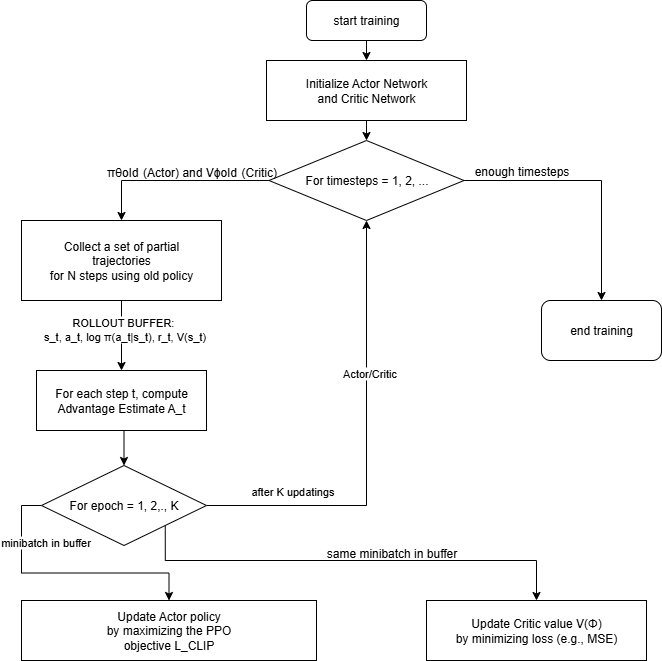
\includegraphics[width=0.7\textwidth]{figures/PPO_training_manual.png}
%     \caption{The PPO training loop data flow. At each iteration, the current policy collects experience into a rollout buffer. Then, advantages are computed, and for several epochs, the actor and critic networks are updated using mini-batches sampled from this buffer.}
%     \label{fig:training_flow}
% \end{figure}

% --- LaTeX Algorithm Code Starts Here ---
\begin{algorithm}[htbp]
\caption{PPO with GAE for Knapsack Problem Training}
\label{alg:ppo}

\SetKwComment{Comment}{\textit{\#}}{}
\SetKwInput{KwPhase}{Phase 1}

% --- Phase 1: Initialization ---
\KwPhase{Initialization}{
    Initialize actor network $\pi_\theta(a|s)$ and critic network $V_\phi(s)$ with shared encoder\;
    Initialize Adam optimizers for parameters $\theta$ and $\phi$\;
    Initialize $N$ parallel `KnapsackEnv` environments\;
}

\BlankLine

\For{each training iteration}{
    
    % --- Phase 2: Rollout (was 2a) ---
    \Comment{--- Phase 2: Rollout / Data Collection ---}
    Initialize an empty Rollout Buffer $\mathcal{D}$\;
    \For{$t = 1 \to \text{n\_steps}$}{
        \For{each parallel environment $i = 1 \to N$}{
            Observe state $s_t^{(i)}$\;
            Sample action $a_t^{(i)} \sim \pi_{\theta_{\text{old}}}( \cdot | s_t^{(i)})$\;
            Compute value $V_\phi(s_t^{(i)})$ and log-probability $\log \pi_{\theta_{\text{old}}}(a_t^{(i)}|s_t^{(i)})$\;
            Execute action $a_t^{(i)}$ to get next state $s_{t+1}^{(i)}$ and reward $r_t^{(i)}$\;
            Let $\tau_t^{(i)} = (s_t^{(i)}, \dots, \log \pi_{\theta_{\text{old}}}(a_t^{(i)}|s_t^{(i)}))$\;
            Store transition $\tau_t^{(i)}$ in $\mathcal{D}$\;
        }
    }
    
    \BlankLine
    % --- Phase 3: Advantage Estimation (was 2b) ---
    \Comment{--- Phase 3: Advantage and Return Estimation ---}
    Compute GAE advantage estimates $\hat{A}_t$ for all transitions in $\mathcal{D}$\;
    Compute returns-to-go $R_t \leftarrow \hat{A}_t + V_\phi(s_t)$ for all transitions in $\mathcal{D}$\;
    
    \BlankLine
    % --- Phase 4: Optimization (was 2c) ---
    \Comment{--- Phase 4: Optimization ---}
    \For{$k = 1 \to \text{n\_epochs}$}{
        \For{each mini-batch of $(s, a, R, \hat{A}, \log \pi_{\text{old}})$ from $\mathcal{D}$}{
            Calculate ratio: $r(\theta) \leftarrow \exp(\log \pi_\theta(a|s) - \log \pi_{\text{old}})$\;
            $L^{\text{CLIP}}(\theta) \leftarrow -\mathbb{E} \left[ \min(r(\theta)\hat{A}, \text{clip}(r(\theta), 1-\epsilon, 1+\epsilon)\hat{A}) \right]$\;
            $L^{\text{VF}}(\phi) \leftarrow \mathbb{E} \left[ (V_\phi(s) - R)^2 \right]$\;
            $S[\pi_\theta] \leftarrow \mathbb{E} \left[ \text{Entropy}(\pi_\theta(s)) \right]$\;
            $L(\theta, \phi) \leftarrow L^{\text{CLIP}}(\theta) + c_1 L^{\text{VF}}(\phi) - c_2 S[\pi_\theta]$\;
            Update parameters $\theta, \phi$ by descending the gradient $\nabla_{\theta,\phi} L(\theta, \phi)$\;
        }
    }
}
\end{algorithm}
% --- LaTeX Algorithm Code Ends Here ---

